\begin{activite}[Un carré sans coins]

\begin{minipage}[c]{0.28\linewidth}
 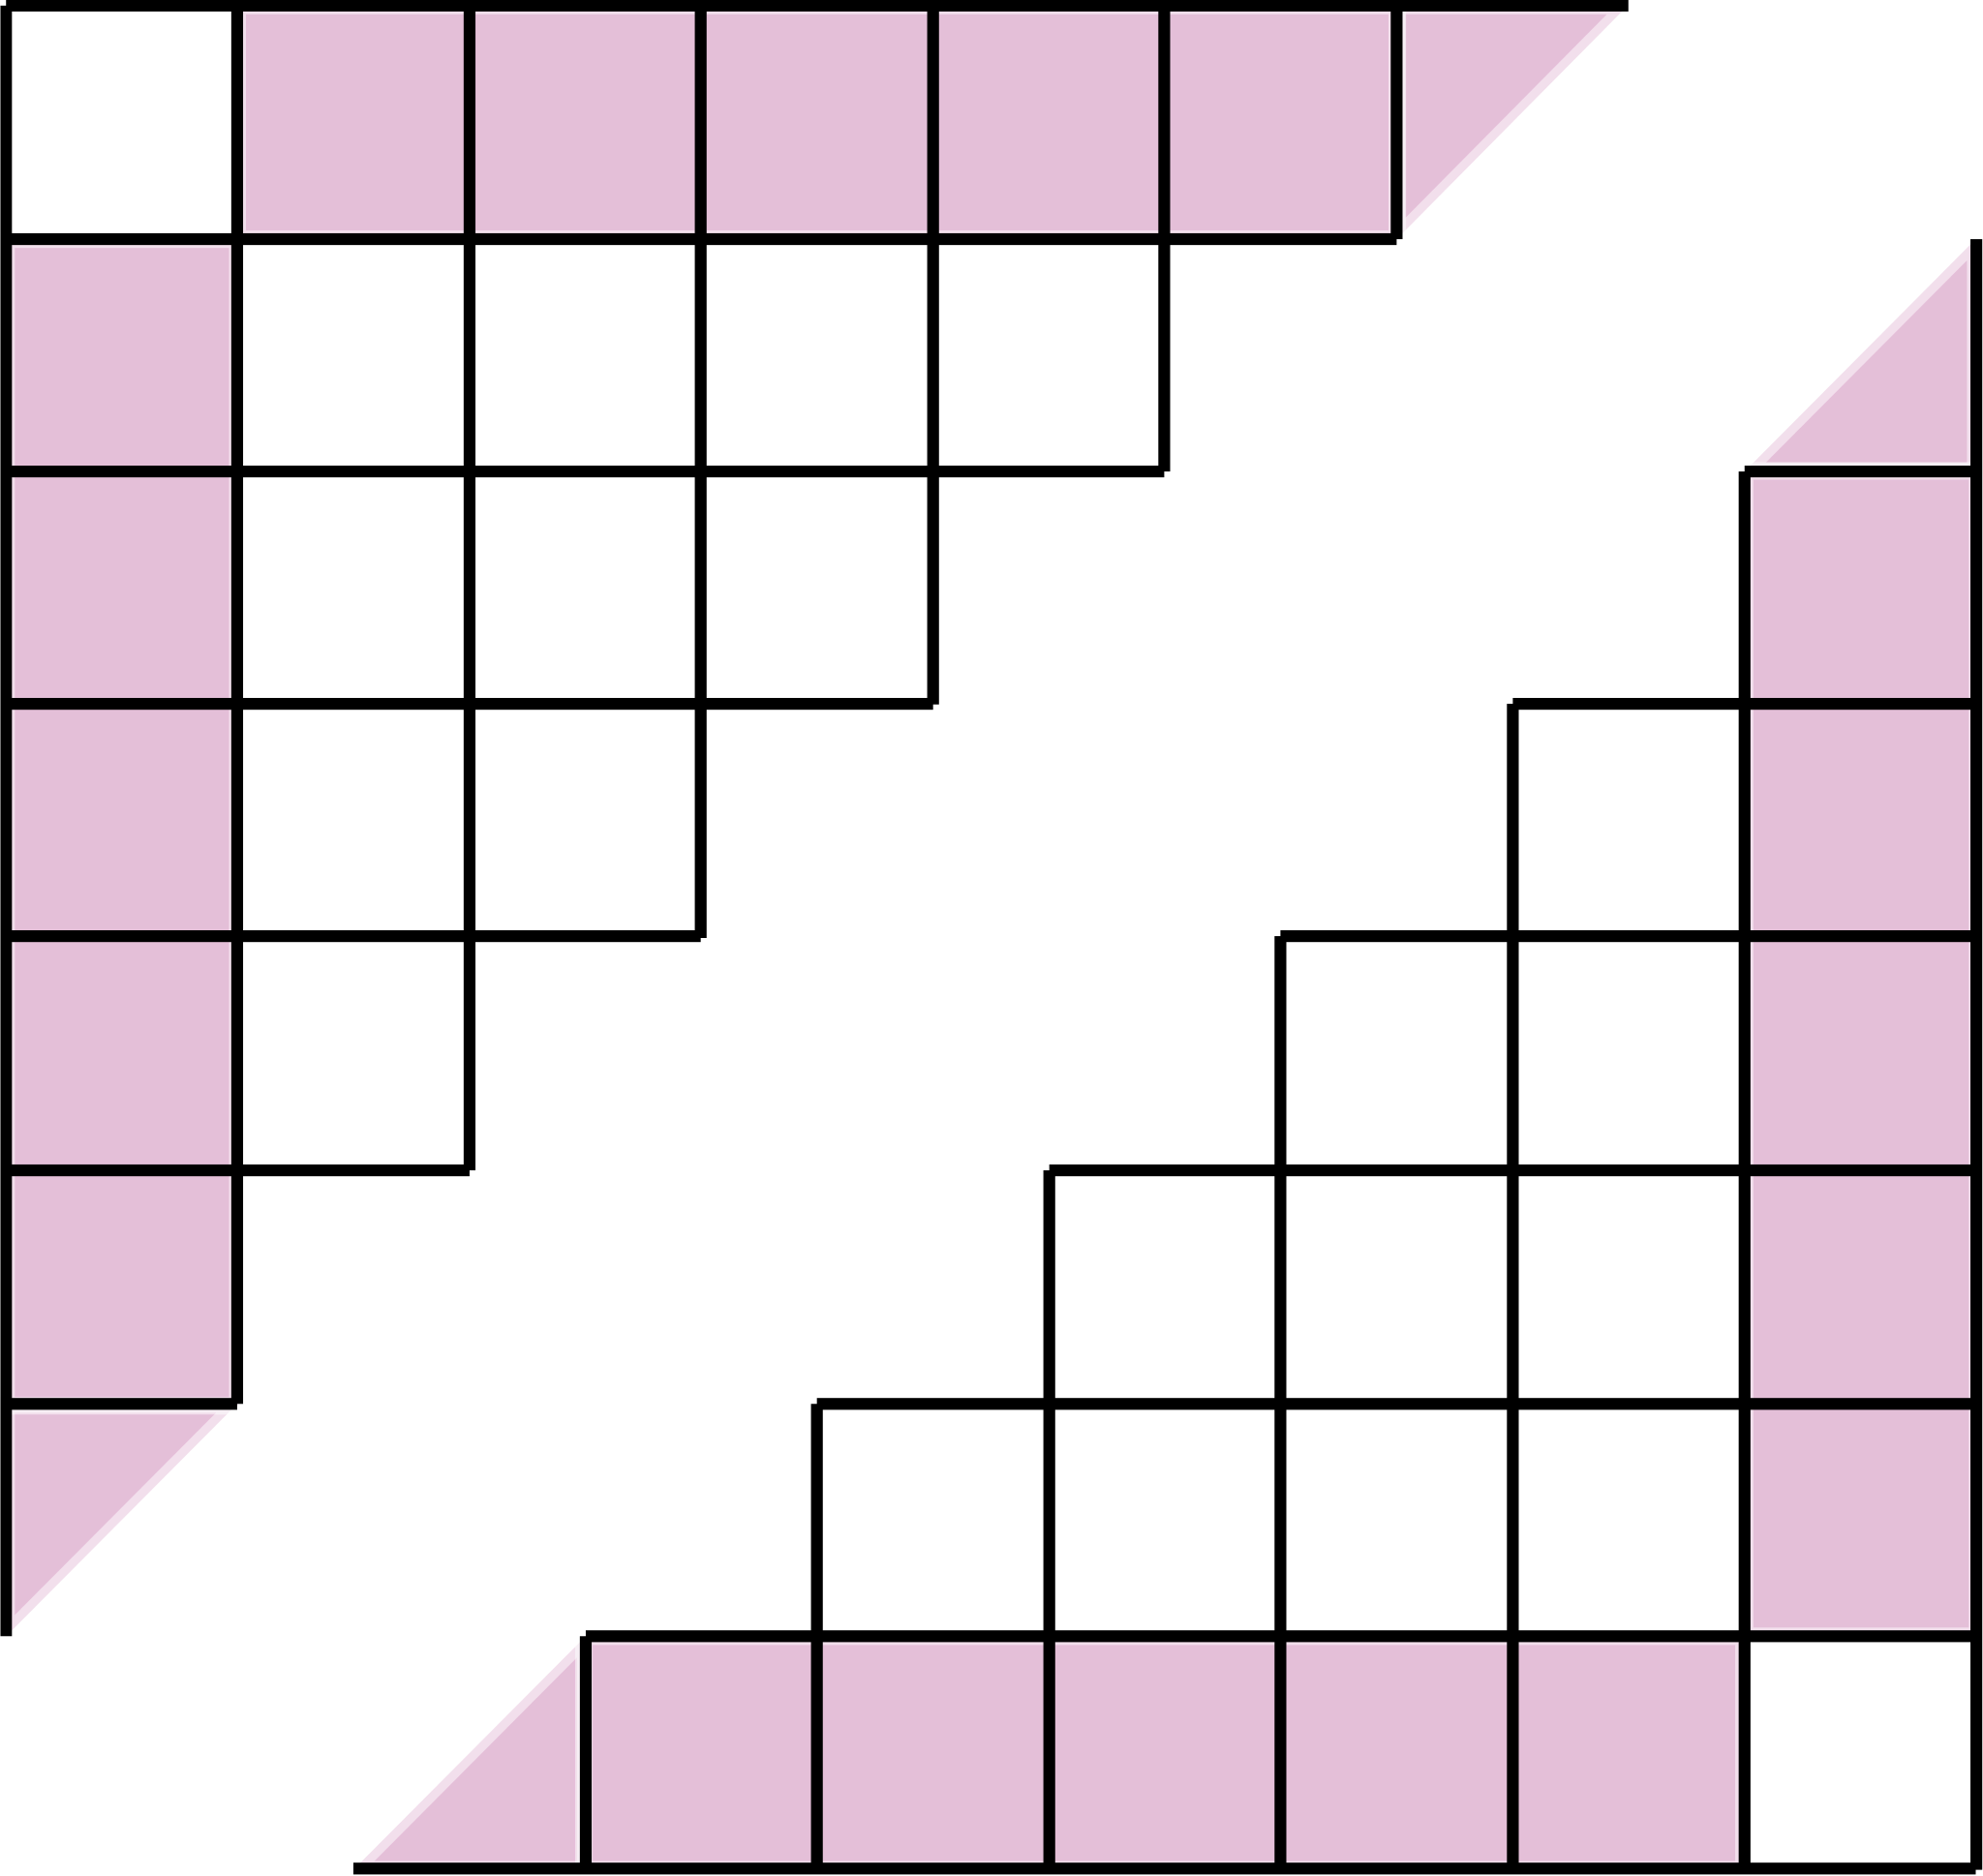
\includegraphics[width=2.5cm]{parties_carre}
 \end{minipage} \hfill
 \begin{minipage}[c]{0.68\linewidth}
On a représenté ci-contre deux parties d'un carré. Il est constitué de petites cases ayant pour côté un carreau. Celles qui se trouvent sur les bords sont coloriées en rose, sauf les quatre coins.
  \end{minipage} \\

\begin{partie}
Réalise une figure de 3 carreaux de côté. Indique le nombre de cases roses. Recommence avec un carré de 4 carreaux de côté puis avec un carré de 5 carreaux de côté.
\end{partie}

\begin{partie}
Quel est le nombre de cases roses pour un carré de 6 carreaux de côté ? Et pour 12 carreaux ? Et pour 100 ?
\end{partie}

\begin{partie}
Le professeur appelle $x$ le nombre de carreaux d'un côté du carré et $G$ le nombre de cases roses. Des élèves ont obtenu les expressions suivantes : \\[0.4em]
\begin{center}
 \begin{tabularx}{0.9\linewidth}{X|X|X}
  Anis : $G = x \cdot 4 - 2$ & Chloé : $G = 4 \cdot (x - 2)$ & Enzo : $G = 4 \cdot x - 8$ \\
  Basile : $G = x - 2 \cdot 4$ & Dalila : $G = (x - 2) \cdot 4$ & Florian : $G = 4 \cdot x - 4$ \\
  \end{tabularx}   
 \end{center}
 \vspace{0.3cm}
Parmi ces expressions, lesquelles sont fausses ? Pourquoi ? Y a-t-il plusieurs bonnes réponses ? Justifie.
\end{partie}

\begin{partie}
Calcule le nombre de cases roses lorsque $x = 6$ puis $x = 24$ et enfin pour $x = 100$.
\end{partie}

\end{activite}

%%%%%%%%%%%%%%%%%%%%%%%%%%%%%%%%%%%%%%%%%%%%%%%%%%%%%%%%%%%%%%%%%%%%%%%

\begin{activite}[Rectangles cousins]

\begin{partie}
Calcule le périmètre et l'aire des deux rectangles suivants. Que remarques-tu ?

\begin{minipage}[c]{0.48\linewidth}
 \begin{center} 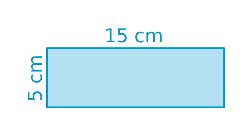
\includegraphics[width=3.8cm]{rect_cousin1} \end{center}
 \end{minipage} \hfill%
 \begin{minipage}[c]{0.48\linewidth}
 \begin{center} 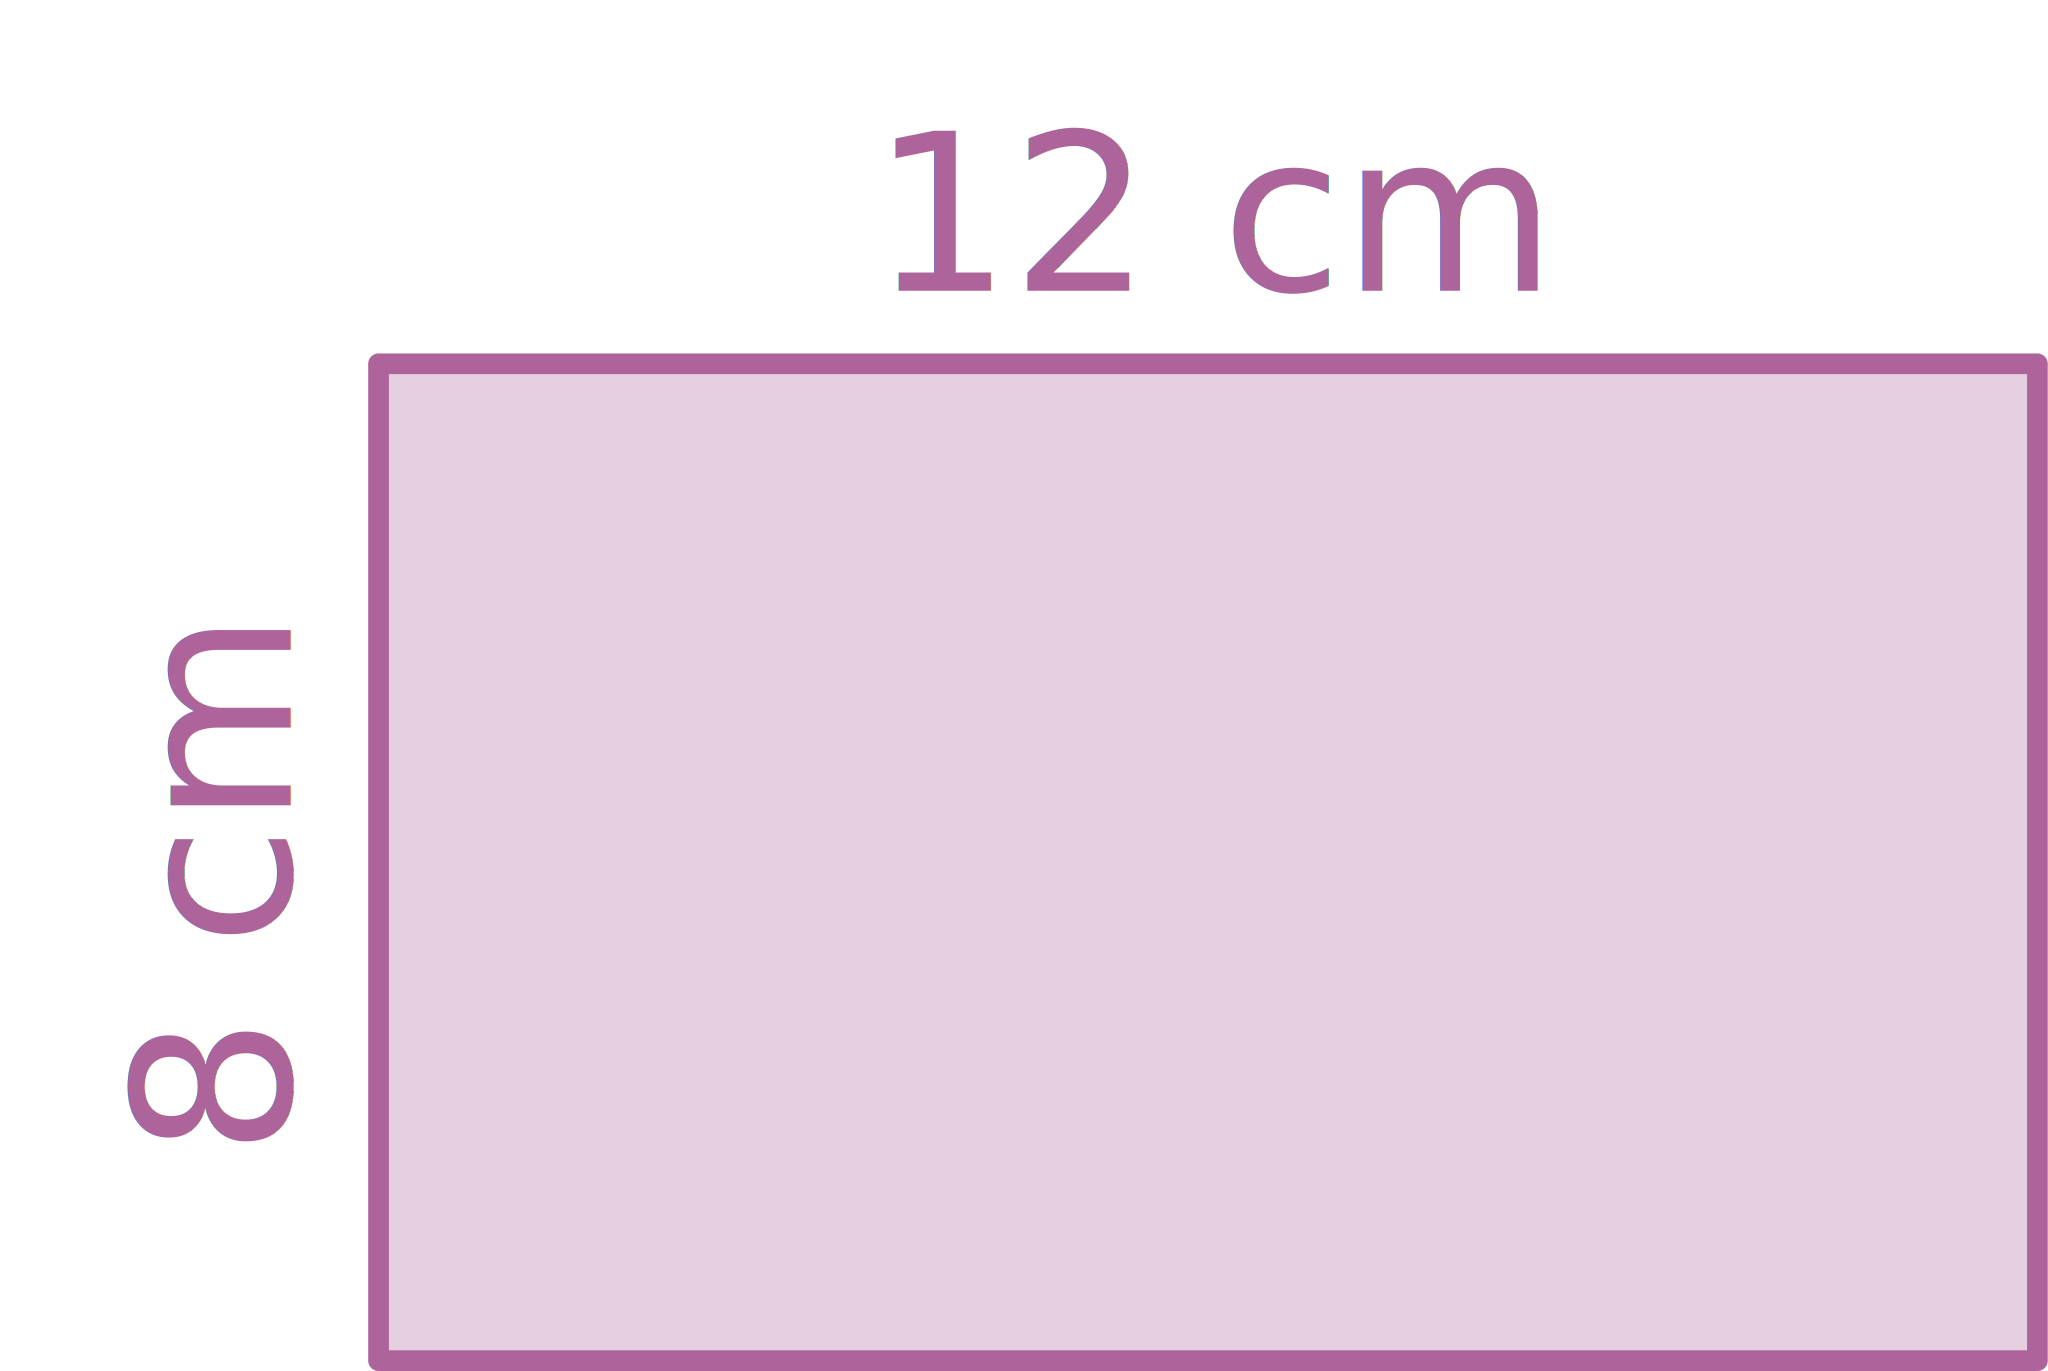
\includegraphics[width=3.3cm]{rect_cousin2} \end{center}
  \end{minipage}\\[0.5em]
Dans cette activité, on s'intéresse uniquement aux rectangles dont le périmètre est 40 cm.
\end{partie}


\begin{minipage}[c]{0.28\linewidth}
 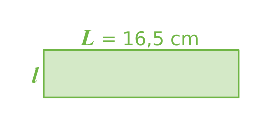
\includegraphics[width=4.3cm]{rect_cousin3}
 \end{minipage} \hfill%
 \begin{minipage}[c]{0.64\linewidth}
\vspace{1em}
\begin{partie}
Un 3\up{e} rectangle a pour longueur $\emph{\textbf{\textcolor{H1}{L}}} = 16,5\,\text{cm}$. Calcule sa largeur $\emph{\textbf{\textcolor{H1}{l}}}$ puis son aire.
\end{partie}

\begin{partie}
Donne les mesures d'un 4\up{e} rectangle de même périmètre.
\end{partie}
  \end{minipage} \\

\begin{partie}
La longueur peut-elle valoir 8 cm ? Et 21 cm ? Justifie et donne les valeurs possibles pour la longueur.
\end{partie}

\begin{partie}
Écris une expression qui permet de calculer la largeur $\emph{\textbf{\textcolor{H1}{l}}}$ en fonction de la longueur $\emph{\textbf{\textcolor{H1}{L}}}$.
\end{partie}

\begin{partie}
En voulant exprimer l'aire du rectangle en fonction de sa longueur $L$, des élèves ont donné les réponses suivantes :
\begin{center}
 \begin{tabularx}{1.1\linewidth}{X|X|X}
  Gaël : $A = L \cdot 20 - L$ & Hamid : $A = L \cdot (20 - L)$ & Karen : $A = 20\,L - L^2$ \\
  Inès : $A = 2 \cdot L + 2 \cdot (20 - L)$ & José : $A = L \cdot 20 - 2 \cdot L$ & Liam: $A = L^2 - 20 \cdot L$ \\
  \end{tabularx}   
 \end{center}
 \vspace{0.3cm}
Parmi ces expressions, lesquelles sont fausses ? Y a-t-il plusieurs bonnes réponses ? Justifie.
\end{partie}

\begin{partie}
Calcule l'aire de ces rectangles pour toutes les valeurs entières de $L$ possibles. Pour quelle valeur de $L$ l'aire semble-t-elle la plus grande ?
\end{partie}

\end{activite}
